\chapter{Macro Tracer}

Macro tracer allows the user to track how HLASM source code is assembled in experience similar to common debugging tools. The user is able to see step by step how CA instructions are interpreted and how macros are expanded.

It is achieved by implementing the Debug Adapter Protocol. The protocol itself is implemented in the language server component, which uses the macro tracer component.

\section{DAP functionality mapping}

The DAP was originally designed to communicate between IDE or editor and debugger or debug adapter. For example, when debugging a C++ application in Visual Studio Code, the editor communicates through DAP with a debugger which is attached to a compiled C++ application.  Contrary to this, macro tracer does not run with compiled binary, it only uses analyzer to simulate the compilation process of high level assembler.

However even though we are not implementing real debugger, it makes very good sense to use debugging interface for tracing the simulation.
\begin{itemize}
	\item \textbf{Instruction pointer} Instruction pointer is commonly showed in debuggers by highlighting line of code which is going to be executed next. This is applicable to HLASM without change, since all the instructions are processed one by one in well defined order.
	\item \textbf{Breakpoints} The user can set a breakpoint when he is interested in tracing only particular section of code. The compilation simulation will stop when it reaches line with breakpoint.
	\item \textbf{Continue} The user can restart stopped simulation by using continue function just as in any debugger.
	\item \textbf{Step in and step over} In debuggers, it is possible to use step in / step over functions to debug implementation of subroutines or skip it and continue after the application returns from the subroutine. In HLASM, this can be applied to macros and COPY instructions: if the user is interested in what happens inside a macro or COPY file, he can use step in. Step over skips to the next instruction in the same file.
	\item \textbf{Variables} The same way common debuggers show values of runtime variables, the macro tracer uses the same functionality to show values of set symbols, macro parameter values and ordinary symbols. It is also possible to visualize attributes of symbols.
	\item \textbf{Call stack} Call stack makes sense with macro tracer too. It can show the stack of currently processed macros and COPY files. Moreover, macros have local set symbols and parameters, so each stack frame may show a different set of valid variables.
\end{itemize}
All described functionality (and more) is supported by the DAP. 
  
\section{Macro tracer architecture}
\begin{figure}
	\centering
	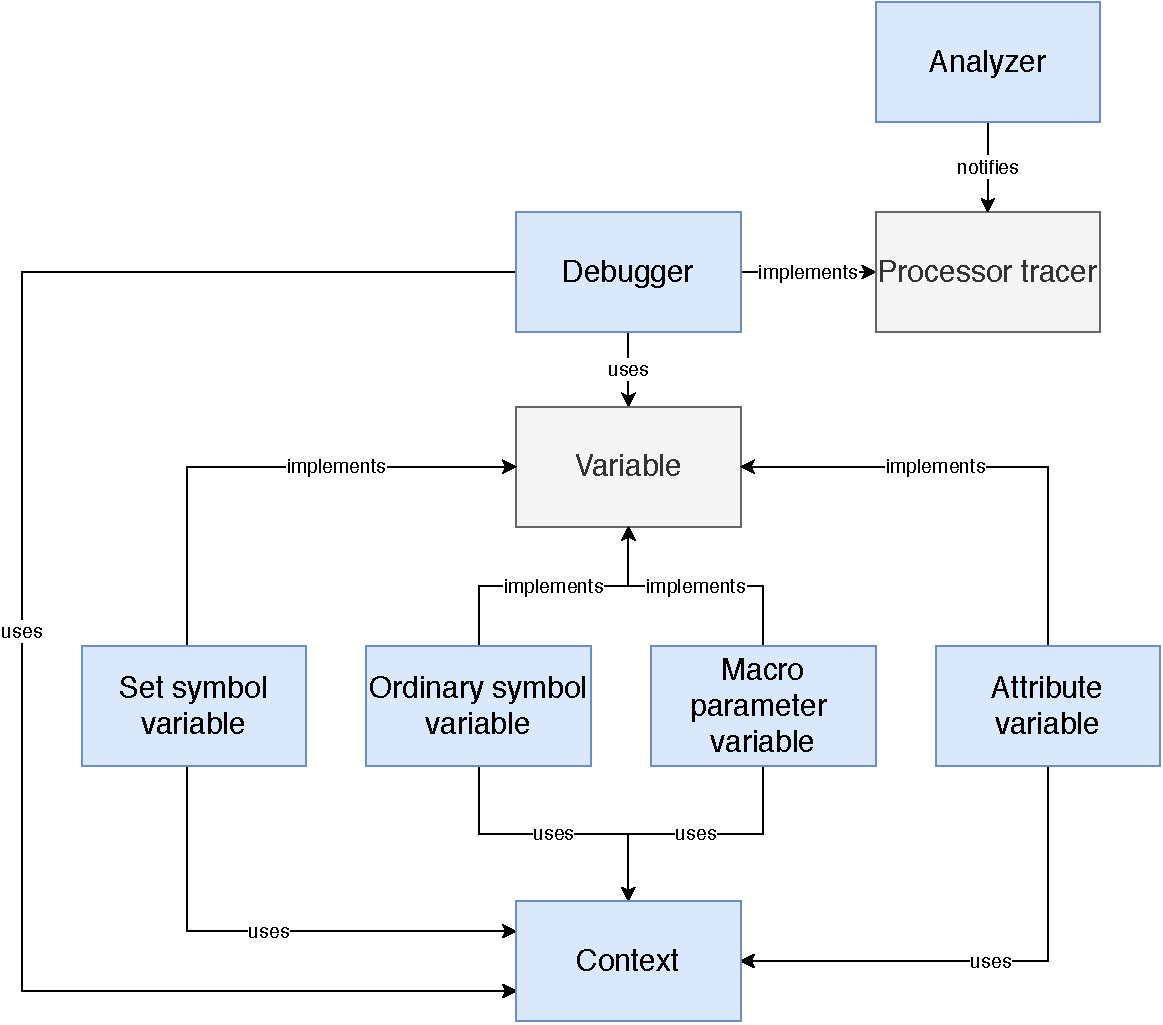
\includegraphics[width=\textwidth]{img/macro_tracer_arch}
	\caption{Architecture of macro tracer.}
	\label{macro_tracer_arch}
\end{figure}

Macro tracer architecture is shown in \cref{macro_tracer_arch}.

Debugger is a class that encapsulates all macro tracer functionality. It starts standard analysis that is provided by the analyzer component in a special thread. The debugger implements processor tracer interface which allows it to receive a notification every time when a statement is about to be processed.

It is also debugger responsibility to extract data from the context used by the analyzer and transform them to a form compatible with DAP.

Debugger uses interface variable which represents a variable as it is shown to the user --- most importantly it is a name-value pair. The variable interface has four implementations:
\begin{itemize}
	\item Set symbol variable
	\item Ordinary symbol variable
	\item Macro parameter variable
	\item Attribute variable
\end{itemize}
Each of the first three represent a HLASM symbol of certain type. They adapt the context representation of the symbols to DAP variables.

Attribute variable represents attributes of all types of symbols. It does not access context, it is only used by the rest of variables to show their attributes.

\section{Debugger}


The debugger component is the core of macro tracer implementation. When the user starts debugging, method \TT{launch} is called from the language server component. The debugger creates analyzer and starts analysis in a separate thread. The debugger implements processor tracer interface which only has one method \TT{statement}. The analyzer calls the \TT{statement} method every time when next statement is about to be processed.

This implementation makes it possible for debugger to stop the analysis using conditional variable. When it sees fit (e.g. when a breakpoint was hit), the debugger can put the thread to sleep and wait for further user interaction. At the same time, it notifies the language server through debug event consumer interface that the analyzer has stopped.

There are three important structures in DAP.
\begin{itemize}
	\item \textbf{Stack frame} Stack frame is one item in call stack. Each frame has name that is shown to the user and points to a line in source code. In macro tracer, each frame points either to the next instruction, to macro call or a COPY instruction.
	\item \textbf{Scope} Each stack frame may have scopes. A scope is simply a group of variables used to make them organized for the user. Macro tracer uses three scopes: Local variables, global variables and ordinary symbols.
	\item \textbf{Variable} Each scope has any number of variables. Each variable has a name and value. They may be further structured and have additional child variables. So DAP can be used to present arbitrary tree of variables to the user. \Cref{dap_nested_variables} shows an example regarding nested macro parameters.

\end{itemize}

\begin{listing}
	
	\begin{verbatim}
	MAC (foo,((bar,ex),am),ple,(lorem,ipsum))
	
	1: foo
	2: ((bar,ex),am)
	1: (bar,ex)
	1: bar
	2: ex
	2: am
	3: ple
	4: (lorem,ipsum)
	1: lorem
	2: ipsum
	
	\end{verbatim}
	\caption{An example how macro tracer leverages DAP nested variables. First line shows a macro call with a parameter. HLASM treats such parameters as nested arrays. Second part shows how such parameter is shown in VS Code using nested variables}
	\label{dap_nested_variables}
\end{listing}

While the thread is stopped, the editor sends requests to display informations about current context. It is the debugger responsibility to extract list of stack frames from the context, return list of scopes for each stack frame and list of variables for each scope. It does not have to deal with complexity of different types of set symbols and macro parameters, that is done by implementations of the variable interface.


